% Document configuration 

\documentclass{beamer}

\usepackage[utf8]{inputenc}
\usepackage{listings}
\usepackage{xcolor}
\usepackage{amsfonts}
\usepackage{graphicx}

% Color definitions
\definecolor{codegreen}{rgb}{0,0.6,0}
\definecolor{codegray}{rgb}{0.5,0.5,0.5}
\definecolor{codepurple}{rgb}{0.58,0,0.82}
\definecolor{backcolour}{RGB}{240,240,240}

% Define a listing style
\lstdefinestyle{mystyle}{
  backgroundcolor=\color{backcolour}, commentstyle=\color{codegreen},
  keywordstyle=\color{magenta},
  numberstyle=\tiny\color{codegray},
  stringstyle=\color{codepurple},
  basicstyle=\ttfamily\footnotesize,
  breakatwhitespace=false,         
  breaklines=true,                 
  captionpos=b,                    
  keepspaces=true,                 
  numbers=left,                    
  numbersep=5pt,                  
  showspaces=false,                
  showstringspaces=false,
  showtabs=false,                  
  tabsize=2
}

% Set the listing style
\lstset{style=mystyle}

\usetheme{Madrid}

%--------------------------

% Title page setup

\title[Plataforma Digital]
{Logística Urbana para Entrega de Mercadorias}

\subtitle{Plataforma Digital}

\author[Grupo 30, 2LEIC03]
{Guilherme Sequeira, Pedro Ramalho, Tomás Pacheco}

\institute[FEUP]
{
  Faculdade de Engenheria\\
  Universidade do Porto
}

\date[2021/2022 2S]
{Desenho de Algoritmos, 2021/2022, 2º semestre}

%--------------------------

% Display the table of contents at the beginning of each section

\AtBeginSection[]
{
  \begin{frame}
    \frametitle{Conteúdos}
    \tableofcontents[currentsection]
  \end{frame}
}

%--------------------------

%----------------------------------------------

% START DOCUMENT

\begin{document}


% Initialize title page

\frame{\titlepage}


% Initialize table of contents

\begin{frame}
  \frametitle{Conteúdos}
  \tableofcontents
\end{frame}




%-------------------------------------------------------

% Begin section : Descrição do problema

\section{Descrição do problema}

%-------------------------------------------------------

% frame 1
\begin{frame}[fragile]
\frametitle{Descrição do problema}
O objetivo do projeto consiste em implementar a plataforma de uma empresa
de logística urbana, de modo a tornar a sua operação o mais eficiente possível.
Considera-se então a implementação de 3 cenários diferentes, cada um com o seu propósito.

A seguir apresenta-se uma explicação formal e detalhada sobre cada um destes cenários, bem como
as análises temporais e espaciais da sua implementação.
\end{frame}

% End section : Descrição do problema

%-------------------------------------------------------




%-------------------------------------------------------

% Begin section : Cenário 1 - Minimização de Estafetas

\section{Cenário 1 - minimização de estafetas}

% frame 1
\begin{frame}
\frametitle{Formalização do problema}
\begin{block}{Descrição}
Dado um conjunto de estafetas $E$, de tamanho $m$, cada um com volume máximo $V_{e}$ e peso máximo $W_{e}$,
e um conjunto de pedidos $P$, de tamanho $n$, cada um com volume $v_{p}$ e peso $w_{p}$, pretende-se
maximizar o número de pedidos entregues, minimizando o número de estafetas contratados.  
\end{block}

Seja $I_{p}$ a variável que representa a inclusão da entrega $p \in P$, $C_{e}$ a variável que representa
a contratação do estafeta $e \in E$, e $x_{ep}$ a variável que determina se o pedido $p$ é entregue pelo estafeta $e$.\\

\begin{enumerate}
\setlength\itemsep{1em}
\item{Objetivo}

\textbf{maximizar} $ \sum_{p = 1}^{n} I_{p} $ 
\hspace{3cm} \textbf{minimizar} $ \sum_{e = 1}^{m} C_{e} $

\item{Restrições}
\begin{itemize}
  \item $ w_{p}, W_{e}, v_{p}, V_{e} \in \mathbb{Z}^{+}$  
  \item $ C, I, x \in \{ 0, 1 \} $
  \item $ W_{e} \geq \sum_{p = 1}^{n} w_{p}x_{ep}, $ $ V_{e} \geq \sum_{p = 1}^{n} v_{p}x_{ep} $
\end{itemize}

\end{enumerate}

\end{frame}

% frame 2
\begin{frame}[fragile]
\frametitle{Descrição do algoritmo}
Em baixo encontra-se pseudocódigo para o algoritmo usado no cenário 1:\\
\begin{lstlisting}[language=python]
sort(estafetas, ordem decrescente, por valor)
sort(pedidos, ordem decrescente, por valor)

for pedido in pedidos:
  for estafeta in estafetas:
    if pedido fits in estafeta:
      estafeta.add_pedido(pedido)
      break
\end{lstlisting}
\end{frame}

% frame 3
\begin{frame}
\frametitle{Análise da complexidade}
Relembrando que $m$ indica o número de estafetas e $n$ indica o número de pedidos, o algoritmo anterior
possui complexidade:\\ 
\centerline{$O(nlog(n) + mlog(m) + mn)$}

\begin{figure}
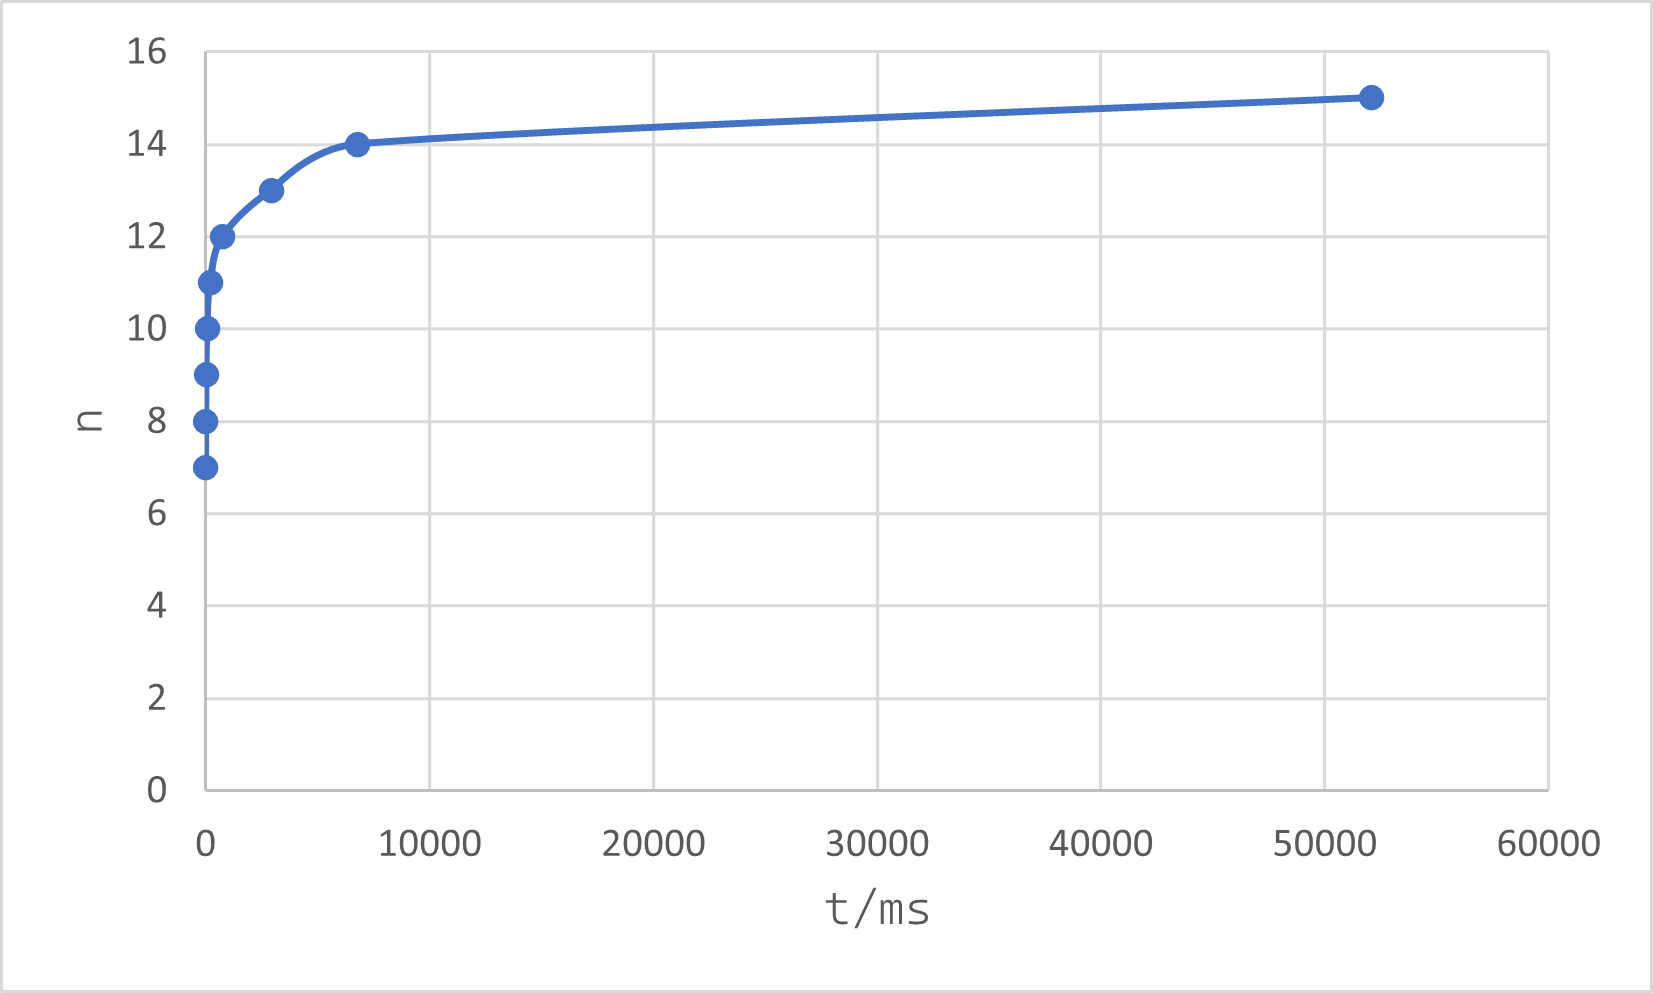
\includegraphics[width=0.5\linewidth]{assets/scenario1.png}
\end{figure}

\textit{Observação: para um valor $n = k$ haverá $2^{k}$ estafetas e $ 9 \times 2^{k}$ pedidos.}

\end{frame}

% frame 4
\begin{frame}
\frametitle{Resultados da avaliação empírica}
\begin{alertblock}{Problema}
É necessário atribuir um critério de prioridade aos estafetas e aos pedidos. Como obter tal critério?
\end{alertblock}

Inicialmente, começamos por chamar a este critério de "valor". Assim, cada estafeta e pedido 
possui um valor associado.
A primeira iteração do algoritmo definia o valor de um estafeta e pedido da seguinte forma:\\
\centerline{$val_{e} = min(w_{e}/w_{t}, v_{e}/v_{t})$      $val_{p} = min(w_{p}/w_{t}, v_{p}/v_{t})$,}

onde $w_{t}$ e $v_{t}$ representam o peso e volume ocupado por todos os pedidos, respetivamente.

Desta forma, o algoritmo seria capaz de ajustar a prioridade dada aos estafetas selecionados de acordo com a necessidade de peso ou volume mais predominante nos pedidos.
Após várias iterações observou-se que $val_{e} = w_{e} + v_{e}$ e $val_{p} = w_{p} + v_{p}$ obteve os melhores resultados.
\end{frame}

% End section : Cenário 1 - Minimização de Estafetas

%-------------------------------------------------------




%-------------------------------------------------------

% Begin section : Cenário 2 - Maximização dos Lucros

\section{Cenário 2 - maximização dos lucros}

% frame 1
\begin{frame}
  \frametitle{Formalização do problema}
  Super important text.
\end{frame}

% frame 2
\begin{frame}
  \frametitle{Descrição dos algoritmos}
  Super important text.
\end{frame}

% frame 3
\begin{frame}
  \frametitle{Análise da complexidade}
  Super important text.
\end{frame}

% frame 4
\begin{frame}
  \frametitle{Resultados da avaliação empírica}
  Super important text.
\end{frame}

% End section : Cenário 2 - Maximização dos Lucros

%-------------------------------------------------------




%-------------------------------------------------------

% Begin section : Cenário 3 - Minimização do Tempo de Entrega

\section{Cenário 3 - minimização do tempo de entrega}

% frame 1
\begin{frame}
  \frametitle{Formalização do problema}
  Super important text.
\end{frame}

% frame 2
\begin{frame}
  \frametitle{Descrição dos algoritmos}
  Super important text.
\end{frame}

% frame 3
\begin{frame}
  \frametitle{Análise da complexidade}
  Super important text.
\end{frame}

% frame 4
\begin{frame}
  \frametitle{Resultados da avaliação empírica}
  Super important text.
\end{frame}

% End section : Cenário 3 - Minimização do Tempo de Entrega

%-------------------------------------------------------




%-------------------------------------------------------

% Begin section : Destaque de Algoritmo

\section{Destaque de algoritmo}

% frame 1
\begin{frame}[fragile]
\frametitle{Destaque de algoritmo}
Algoritmo super broken goes here.
\end{frame}

% End section : Destaque de Algoritmo

%-------------------------------------------------------



%-------------------------------------------------------

% Begin section : Principais dificuldades

\section{Principais dificuldades}

% frame 1
\begin{frame}
\frametitle{Principais dificuldades}
Dificuldades encontradas go here.

\end{frame}

% End section : Principais dificuldades

%-------------------------------------------------------



%-------------------------------------------------------

% Begin section : Esforço do Grupo

\section{Esforço do grupo}

% frame 1
\begin{frame}
\frametitle{Esforço do grupo}
Esforço do grupo goes here.
\end{frame}

% End section : Esforço do Grupo

%-------------------------------------------------------




%-------------------------------------------------------

% Begin section : Outras observações

\section{Outras observações}

% frame 1
\begin{frame}
\frametitle{Explicação do \textit{dataset} gerado}
Explicação sobre o dataset gerado goes here.
\end{frame}

% frame 2
\begin{frame}
\frametitle{Referências}
Referências go here.
\end{frame}

% End section : Outras observaçṍes

%-------------------------------------------------------


\end{document}
